\documentclass[submit]{harvardml}

% Put in your full name and email address.
\name{Aditya Prasad}
\email{adityaprasad@college.harvard.edu}

% List any people you worked with.
\collaborators{%
 None
}


% You don't need to change these.
\course{CS281-F17}
\assignment{Assignment \#0, v 1.0}
\duedate{5:00pm Sept. 8th}
\newcommand{\attr}[1]{\textsf{#1}}
\usepackage[OT1]{fontenc}
\usepackage[colorlinks,citecolor=blue,urlcolor=blue]{hyperref}
\usepackage[pdftex]{graphicx}
\usepackage{fullpage}
\usepackage{palatino}
\usepackage{amsfonts}
\usepackage{amsmath}
\usepackage{amssymb}
\usepackage{color}
\usepackage{todonotes}
\usepackage{listings}
\usepackage{common}
\usepackage{bm}
\usepackage{enumitem}
\usepackage{tikz}
\usepackage{xifthen}
\usepackage{soul}
\usepackage{url}
\usepackage[mmddyyyy,hhmmss]{datetime}
\definecolor{verbgray}{gray}{0.9}
% Some useful macros.
\newcommand{\R}{\mathbb{R}}
\newcommand{\E}{\mathbb{E}}
\newcommand{\cov}{\text{cov}}
\renewcommand{\v}[1]{\mathbf{#1}}

\begin{document}
\begin{center}
    {\Large Homework 0: Preliminary}
\end{center}

%\subsection*{Introduction}

There is a mathematical component and a programming component to this homework.
Please submit your PDF and Python files to Canvas, and push all of your work
to your GitHub repository. If a question requires you to make any plots,
please include those in the writeup.

This assignment is intended to ensure that you have the background required for CS281,
and have studied the mathematical review notes provided in section.
You should be able to answer the problems below \textit{without} complicated calculations.
All questions are worth $70/6 = 11.\bar{6}$ points unless stated otherwise.

\newpage



%%%%%%%%%%%%%%%%%%%%%%%%%%%%%%%%%%%%%%%%%%%%%%%%%%%%%%%%
%%%%%%%%%%%%%%%%%% PROBLEM 1 %%%%%%%%%%%%%%%%%%%%%%%%%%%
%%%%%%%%%%%%%%%%%%%%%%%%%%%%%%%%%%%%%%%%%%%%%%%%%%%%%%%%
\section*{Variance and Covariance}
\begin{problem}
Let $X$ and~$Y$ be two independent random variables.

\begin{enumerate}[label=(\alph*)]
\item Show that the independence of~$X$ and~$Y$ implies that their
covariance is zero.

\item Zero covariance \textit{does not} imply independence between two
      random variables. Give an example of this.

\item For a scalar constant~$a$, show the following two properties:
\begin{align*}
  \E(X + aY) &= \E(X) + a\E(Y)\\
  \var(X + aY) &= \var(X) + a^2\var(Y)
\end{align*}
\end{enumerate}
\end{problem}

\begin{enumerate}[label=(\alph*)]
	\item $X \perp Y$. Therefore, we have:
		\begin{align}
			Cov(X, Y) &= E((X - E(X))(Y-E(Y)) \\
					&= E(X - E(X)) E(Y-E(Y)) \\
					&= 0
		\end{align}
		Alternatively, we have:
		\begin{align}
			Cov(X,Y) &= E(XY) - E(X)E(Y) - E(X E(Y)) + E (Y E(X)) \\
					&= 2 E(X) E(Y) - 2E(X) E(Y)  = 0
		\end{align}
		
		Here, we have assumed the general result that if two random variables are independent, the expectation of the product is then the product of the expectation.
	
	\item Covariance is a measure of linear association; therefore, consider some solely non-linear dependence: $Y = X^2, X \sim N(0,1)$. To heuristically see why there isn't any covariance, consider moving across the possible values of X from $-\infty$ to $\infty$. First an increase in $X$ is associated with a decrease in $Y$. But after crossing $X=0$, an increase in $X$ is associated with an increase in $Y$. Overall, however, these two effects essentially cancel out.
		\begin{align}
			Cov(X,Y) &= E(X Y) - E(X) E(Y) \\
					&= E(X^3) - E(X)E(X^2) \\
					&= 0 - 0 = 0
		\end{align}
		
		$Y$ and $X$ are obviously not independent, but they are uncorrelated.
		
	\item Consider two random variable $X$ and $Y$. Here, we assume that they are continuous. The pdf of $X$ is $f_X$, and that of $Y$ is $f_Y$. Therefore, $X + aY$ is distributed as $f_{X,Y}$ (the joint pdf of $X$ and $Y$). Therefore, we have:
		\begin{align}
			E(X + aY) &= \int_{-\infty}^{\infty}\int_{-\infty}^{\infty} {(x + a y) f_{X,Y} (x,y) dx dy} \\
					&=  \int_{-\infty}^{\infty}{x dx}\int_{-\infty}^{\infty}{f_{X,Y} (x,y) dy} + a \int_{-\infty}^{\infty}{y dy}\int_{-\infty}^{\infty} {f_{X,Y} (x,y) dx}
		\end{align}
		We have put this in a form where we can simply integrate out the unnecessary terms and move from the joint pdfs to marginal pdfs.
		\begin{align}
			E(X + aY) &= \int_{-\infty}^{\infty}{x f_X (x) dx} + a \int_{-\infty}^{\infty}{y f_Y (y) dy} \\
						&= E(X) + a E(Y)
		\end{align}
		Note, this theorem is true irrespective of whether $X$ and $Y$ are independent. Now, we prove the corresponding theorem for variance, where this is not true.
		
		\begin{align}
			Var(X + aY) &= E((X + aY)^2) - E^2(X + aY) \\
						&= E(X^2 + a^2 Y^2 + 2a XY) - (E(X) + aE(Y))^2 \\
						&= E(X^2) - E^2(X) + a^2 (E(Y^2) - E^2(Y)) + 2a E(XY) - 2a E(X)E(Y) \\
						&= Var(X) + a^2 Var(Y) + 2a Cov(X,Y)
		\end{align}
		If $X \perp Y$, then we have:
		\begin{align}
			Var(X + aY) = Var(X) + a^2 Var(Y)
		\end{align}
\end{enumerate}

\newpage
%%%%%%%%%%%%%%%%%%%%%%%%%%%%%%%%%%%%%%%%%%%%%%%%%%%%%%%%
%%%%%%%%%%%%%%%%%% PROBLEM 2 %%%%%%%%%%%%%%%%%%%%%%%%%%%
%%%%%%%%%%%%%%%%%%%%%%%%%%%%%%%%%%%%%%%%%%%%%%%%%%%%%%%%
\section*{Densities}
\begin{problem}
Answer the following questions:
\begin{enumerate}[label=(\alph*)]
  \item Can a probability density function (pdf) ever take values greater than 1?
  \item Let $X$ be a univariate normally distributed random variable with mean 0
        and variance $1/100$. What is the pdf of $X$?
  \item What is the value of this pdf at 0?
  \item What is the probability that $X = 0$?
  \item Explain the discrepancy.
\end{enumerate}
\end{problem}

\begin{enumerate}[label=(\alph*)]
	\item Yes. The only constraint on a probability density function is that it must integrate to 1. An obvious display of this is the following uniform distribution, $f_X (x) = 2, x \in [0, 1/2]$. A neater description of this is the Dirac-delta distribution, which essentially represents certainty about an event.
	
	\item The pdf is:
		\begin{align}
			f_X(x) = \frac{1}{\sqrt{2\pi \sigma^2}} \exp\left[-\frac{1}{2} \frac{x^2}{\sigma^2}\right]
		\end{align}
		where $\sigma^2 = 1/100$.
	
	\item $f_X (0) =  \frac{1}{\sqrt{2\pi}\sigma} = \frac{10}{\sqrt{2\pi}}$
	\item $P(X=0) = \int_{0}^{0}{f_X(x) dx} = 0$
	\item The set $X=0$ is of volume 0; therefore, the probability that it happens is zero (given that we're integrating over a set of volume zero). More intuitively, given that there an un-countably infinite number of reals between $X= -\infty \rightarrow \infty$, the probability that $X$ equals exactly $0$ is $0$. 
	
	A better framed-question would to be ask what the probability of $X=0$ is around a small ball of radius $\epsilon > 0$ centered at $X=0$. We then have:
		\begin{align}
			P(X=0) &= -\int_{0-\epsilon}^{0+\epsilon} {f_X(x) dx} \\
					&= \frac{10}{\sqrt{2\pi}} erf(\epsilon)
		\end{align}
		As can be seen, as $\epsilon \rightarrow 0, P(X=0) \rightarrow 0$.
\end{enumerate}
\newpage
%%%%%%%%%%%%%%%%%%%%%%%%%%%%%%%%%%%%%%%%%%%%%%%%%%%%%%%%
%%%%%%%%%%%%%%%%%%%% PROBLEM 3 %%%%%%%%%%%%%%%%%%%%%%%%%
%%%%%%%%%%%%%%%%%%%%%%%%%%%%%%%%%%%%%%%%%%%%%%%%%%%%%%%%
\section*{Conditioning and Bayes' rule}
\begin{problem}
  Let $\v \mu \in \R^m$ and
  $\v \Sigma, \v \Sigma' \in \R^{m \times m}$.  Let $X$ be an
  $m$-dimensional random vector with
  $X \sim \mathcal{N}(\v \mu, \v \Sigma)$, and let $Y$ be a
  $m$-dimensional random vector such that
  $Y \given X \sim \mathcal{N}(X, \v \Sigma')$. Derive the
  distribution and parameters for each of the following.

\begin{enumerate}[label=(\alph*)]
  \item The unconditional distribution of $Y$.

  \item The joint distribution for the pair $(X,Y)$.

\end{enumerate}

Hints:
\begin{itemize}
\item You may use without proof (but they are good advanced exercises)
  the closure properties of multivariate normal distributions. Why is
  it helpful to know when a distribution is normal?
\item Review Eve's and Adam's Laws, linearity properties of
  expectation and variance, and Law of Total Covariance.

\end{itemize}

\end{problem}
\begin{enumerate}[label=(\alph*)]
	\item Given that $Y \mid X$ and $X$ are distributed as Gaussians, from the closure properties of normals, we know that the marginal distribution of $Y$ should also be Gaussian. Therefore, we only need to calculate the mean and variance to fully specify this distribution.
	
	From Adam's law, we have:
	\begin{align}
		E(Y) = E(E(Y|X)) = E(X) = \v{\mu} \in \mathbb{R}^m
	\end{align}
	
	From Eve's law, we have:
	\begin{align}
		Var(Y) &= Var(E(Y|X)) + E(Var(Y|X)) \\
			&= Var(X) + \v{\Sigma^*} \\
			&= \v{\Sigma} + \v{\Sigma^*}
	\end{align}
	
	\item Now we calculate the joint distribution of the vector: $(X,Y)^T$. Given that the marginals are normal, from the closure properties of normals, we know that joint distribution is also distributed as a normal. Therefore, we need to calculate only the mean vector and covariance matrix to specify this distribution. The mean is simply going to be: $(\v{\mu}, \v{\mu}) \in \mathbb{R}^{2m}$. The quadratic form looks like:
	\begin{align}
		(\v{x}, \v{y}) \Sigma_{XY}^{-1} (\v{x}, \v{y})^T
	\end{align}
	We know that the covariance matrix for such a system looks like:
	$$\begin{pmatrix}
		Var(X) && Cov(X,Y) \\
		Cov(Y,X) && Var(Y)
	\end{pmatrix}$$
	We know $var(X) = \Sigma$ and $var(Y) = \Sigma + \Sigma^*$. We also know that $Cov(X,Y) = Cov(Y,X)$. We now calculate $Cov(X,Y)$. From the law of total covariance, we have:
	\begin{align}
		Cov(X,Y) &= E(Cov(X,Y|Z)) + Cov(E(X|Z), E(Y|Z))
	\end{align}
	Let $Z=X$. Then, we have:
	\begin{align}
		Cov(X,Y) &= E(Cov(X,Y|X)) + Cov(X, X) \\
				&= 0 + Var(X)
	\end{align}
	Another way to do calculate $Cov(X,Y)$ is through the definition:
	\begin{align}
		Cov(X,Y) &= E(XY) - E(X)E(Y) \\
				&= E_{X} \left[X E_{Y|X} \left[Y\right]\right] - E(X)E(Y) \\
				&= E_X [X^2] - E(X) E(X) \\
				&= Var(X)
	\end{align}
	Also, because of symmetry: $Cov(Y,X) = Cov(X,Y)$. Therefore, we have fully specified the matrix:
	$$\begin{pmatrix}
		\v{\Sigma} && \v{\Sigma} \\
		\v{\Sigma} && \v{\Sigma} + \v{\Sigma^{'}}
	\end{pmatrix}$$
\end{enumerate}
\newpage
%%%%%%%%%%%%%%%%%%%%%%%%%%%%%%%%%%%%%%%%%%%%%%%%%%%%%%%%
%%%%%%%%%%%%%%%%% PROBLEM 4 %%%%%%%%%%%%%%%%%%%%%%%%%%%%
%%%%%%%%%%%%%%%%%%%%%%%%%%%%%%%%%%%%%%%%%%%%%%%%%%%%%%%%
\section*{I can Ei-gen}
\begin{problem}
    Let $\v X \in \R^{n \times m}$.
    \begin{enumerate}[label=(\alph*)]
        \item What is the relationship between the $n$ eigenvalues
              of $\v X \v X^T$ and the $m$ eigenvalues of $\v X^T \v X$?
        \item Suppose $\v X$ is square (i.e., $n=m$) and symmetric.
              What does this tell you about the eigenvalues of $\v X$?
              What are the eigenvalues of $\v X + \v I$, where $\v I$ is the identity matrix?
        \item Suppose $\v X$ is square, symmetric, and invertible.
			  What are the eigenvalues of $\v X^{-1}$?
	\end{enumerate}
	Hints:
	\begin{itemize}
		\item Make use of singular value decomposition and the properties
			  of orthogonal matrices. Show your work.
		\item Review and make use of (but do not derive) the spectral theorem.
	\end{itemize}
\end{problem}

\begin{enumerate}[label=(\alph*)]
	\item Any $X \in \mathbb{R}^{m \times n}$ admits a singular value decomposition. Thus, we can write $X$ as follows:
		\begin{align} \centering
			X = \Sigma U V^T
		\end{align}
		Here, $\Sigma$ and $V$ are orthogonal matrices, while $U$ is a diagonal matrix. Now, consider $X X^T$. We write this out using the singular value decomposition:
	\begin{align} \centering
		X X^T &= (\Sigma U V^T) (V U^T \Sigma^T)\\
			&= \Sigma U (V^T V) U^T \Sigma^T\\
			&= \Sigma U U^T \Sigma^T 
	\end{align}				
			
			There are a couple of important things to note: firstly, $X X^T$ is obviously a square symmetric matrix. ($(XX^T)^T = XX^T$). Since (by the spectral theorem for symmetric matrices) every symmetric matrix admit admits a unique eigenvalue decomposition (up to a constant) of the form:
	\begin{align} \centering
		X X^T = P^{-1} D P
	\end{align}
Here, $P$ is an orthogonal eigenbasis matrix, while $D$ is the diagonal eigenvalue matrix (essentially principal axis theorem). Therefore on comparing the two forms above, we can conclude that:
\begin{align} \centering
	D &= U U^T \\
	P^{-1} &= \Sigma
\end{align} 

Therefore, the eigenvalues of $X X^T$ are stored in the diagonal matrix $UU^T$ (the product of two diagonal matrices is another diagonal matrix). The second thing to note here is that because $U$ is diagonal, it is symmetric; that is $U= U^T$. Therefore, 
\begin{align}
	UU^T &= U^2\\
	\implies D &= U^2
\end{align}

We can do a similar spectral decomposition for $X^T X$, and use eigen-decomposition to see its matrix of eigenvalues. 
	\begin{align}
	X^T X &= V U^T \Sigma^T \Sigma U V^T \\
		&= V U^T U V^T \\
		&= V U^2 \Sigma
	\end{align}	 

By the same eigenvalue-decomposition argument as above, we note that the diagonal eigenvalue matrix, $D^{'}$ of $X^T X$ is:
	\begin{align}
		D^{'} = U^2
	\end{align}
\textbf{Therefore, we note that the eigenvalues of the two matrices are the same.} The eigenvectors, however, are generally different. The fact that the eigenvalues are the same seems to relate to the fact that the row rank is the same as the column rank. In other words, the dimension of both spaces is the same. We have essentially constructed an orthonormal basis in either space, and these bases seem to have a similar ``geometric shape" (evinced by their eigenvalues).

	\item If $X \in GL_n(\mathbb{R})$ is symmetric, we know (by the Spectral Theorem) that the eigenvalues of $X$ are real. The eigenvalues of ($X + I$) are essentially each of the eigenvalues plus one. Let $v$ be an eigenvector if $X$. Then:
		\begin{align}
			(X + I) v = (\lambda + 1) v
		\end{align}
	
	\item $X = X^T$. Let $\v{v}$ be an eigenvector of $X$ with eigenvalue $\lambda$. Then:
		\begin{align}
			X \v{v} &= \lambda \v {v}\\
			\implies X^{-1} X \v{v} &= \lambda X^{-1} \v{v} \\
			\implies X^{-1} \v{v} &= \frac{1}{\lambda} \v{v}
		\end{align}
		Therefore, the eigenvalues are each the multiplicate inverse of those of the forward function. This is independent of whether $X$ is symmetric. In essence, the forward function scales each eigenvector, and so the inverse function just scales them back.
\end{enumerate}
\newpage
%%%%%%%%%%%%%%%%%%%%%%%%%%%%%%%%%%%%%%%%%%%%%%%%%%%%%%%%%%
%%%%%%%%%%%%%%%%%%% PROBLEM 5 %%%%%%%%%%%%%%%%%%%%%%%%%%%%
%%%%%%%%%%%%%%%%%%%%%%%%%%%%%%%%%%%%%%%%%%%%%%%%%%%%%%%%%%
\section*{Vector Calculus}
\begin{problem}
  Let $\v x, \v y \in \R^m$ and $\v A \in \R^{m \times m}$. Please derive from
  elementary scalar calculus the following useful properties. Write
  your final answers in vector notation.
\begin{enumerate}[label=(\alph*)]
    \item What is the gradient with respect to $\v x$ of $\v x^T \v y$?
    \item What is the gradient with respect to $\v x$ of $\v x^T \v x$?
    \item What is the gradient with respect to $\v x$ of $\v x^T \v A \v x$?
\end{enumerate}
\end{problem}

\begin{enumerate}[label=(\alph*)]
	\item Consider the inner product: $\langle \v{x}, \v{y} \rangle$. In Einstein notation (two same indices indicate a summation), we have:
	\begin{align}
		\langle \v{x}, \v{y} \rangle = x_i y_i
	\end{align}
	The derivate with respect to $x_j$ is simply:
	\begin{align}
		\partial_{x_j} \langle \v{x}, \v{y} \rangle &= \partial_{x_j}  x_i y_i \\
		&= y_i \delta_{ij} = y_j
	\end{align}
	
	Therefore, the gradient with respect to $\v x$ of $\v x^T \v y$ is simply $\v{y}$.
	
	\item Similarly, we have:
		\begin{align}
			\langle \v{x}, \v{x} \rangle = x_i x_i
		\end{align}
		
		Therefore,
		\begin{align}
		\partial_{x_j} \langle \v{x}, \v{x} \rangle &= \partial_{x_j}  x_i x_i \\
		&= 2 x_i \delta_{ij} = 2 x_j
	\end{align}
	
	Therefore, the gradient with respect to $\v x$ of $\v x^T \v y$ is simply $2 \v{x}$.
	
	\item Assume now that the inner product space is given by the matrix $A$, we have:
		\begin{align}
			\langle \v{x}, \v{x} \rangle = x_i A_{ij} x_j
		\end{align}
		
		Therefore,
		\begin{align}
		\partial_{x_k} \langle \v{x}, \v{x} \rangle &= \partial_{x_k}  x_i A_{ij} x_j \\
		&= \left[A_{ij}x_j \right]\delta_{ik} + \left[A_{ij} x_i \right] \delta_{jk} \\
		&= A_{kj} x_j + A_{ik}x_i \\
		&= A_{kj} x_j + A^T_{ki}x_i \\
		\end{align}
		
		Therefore, in vector notation, the gradient is:
		\begin{align}
			\v{(A + A^T) x}
		\end{align}
		
		It makes sense that the matrix representing the gradient operator in this space is symmetric; the angle of steepest ascent for $\v e_i$, $\v e_j$ should be the same for $\v e_j$, $\v e_i$. 
	
\end{enumerate}
\newpage
%%%%%%%%%%%%%%%%%%%%%%%%%%%%%%%%%%%%%%%%%%%%%%%%%%%%%%%%%%%%
%%%%%%%%%%%%%%%%%%%%% PROBLEM 7 %%%%%%%%%%%%%%%%%%%%%%%%%%%%
%%%%%%%%%%%%%%%%%%%%%%%%%%%%%%%%%%%%%%%%%%%%%%%%%%%%%%%%%%%%
\section*{Gradient Check}
\begin{problem}
  Often after finishing an analytic derivation of a gradient, you will
  need to implement it in code.  However, there may be mistakes -
  either in the derivation or in the implementation. This is
  particularly the case for gradients of multivariate functions.

  \air

  \noindent One way to check your work is to numerically estimate the gradient
  and check it on a variety of inputs. For this problem we consider
  the simplest case of a univariate function and its derivative.  For
  example, consider a function $f(x): \mathbb{R} \to \mathbb{R}$:
$$\frac{d f}{d x} = \underset{\epsilon \to 0} \lim \frac{f(x + \epsilon) - f(x - \epsilon)}{2 \epsilon}$$
\noindent A common check is to evaluate the right-hand side for a small value of
$\epsilon$, and check that the result is similar to your analytic
result.\\

\smallskip

\noindent In this problem, you will implement the analytic and numerical derivatives of the function \[f(x) = \cos(x) + x^2 + e^x.\]

\begin{enumerate}
  \item Implement \texttt{f} in Python (feel free to use whatever \texttt{numpy} or \texttt{scipy} functions you need):
  \begin{lstlisting}[language=python]
  def f(x):

  \end{lstlisting}
  \item Analytically derive the derivative of that function, and implement it in Python:
  \begin{lstlisting}[language=python]
  def grad_f(x):
  \end{lstlisting}
  \item Now, implement a gradient check (the numerical approximation to the derivative), and by plotting, 
        show that the numerical approximation approaches the analytic as \texttt{epsilon} 
        $\to 0$ for a few values of $x$:
  \begin{lstlisting}[language=python]
  def grad_check(x, epsilon):

  \end{lstlisting}
\end{enumerate}
\end{problem}

\begin{lstlisting}[language=python]
import numpy as np
import matplotlib.pyplot as plt
\end{lstlisting}
\begin{enumerate}[label=(\alph*)]
	\item \begin{lstlisting}[language=python]
def f(x):
	return np.cos(x) + x**2 + np.exp(x)
		\end{lstlisting}
	
	\item \begin{lstlisting}[language=python]
def grad_f(x):
	return -np.sin(x) + 2.*x + np.exp(x)
		\end{lstlisting}
	
	\item \begin{lstlisting}[language=python]
def grad_check(x, eps):
    return (f(x + eps) - f(x-eps)) / float((2*eps))

def plot():
    xs = [1., 5., 6., 8.,10.]
    eps = np.linspace(0.001,1, 100)
    vect = np.vectorize(grad_check)
    cnt = 0
    plt.figure(figsize=(8,8))
    for x in xs:
        cnt = cnt + 1
        print(cnt)
        plt.xlabel("Epsilon")
        plt.ylabel("Error")
        y = vect(x,eps) - grad_f(x)
        plt.plot(eps, y, label="x = %2.2f"%x)
        plt.legend()
    plt.savefig('plot.pdf', dpi=600, bbox_inches='tight', transparent=False)
		\end{lstlisting}
		
		\begin{figure}[tbh]
			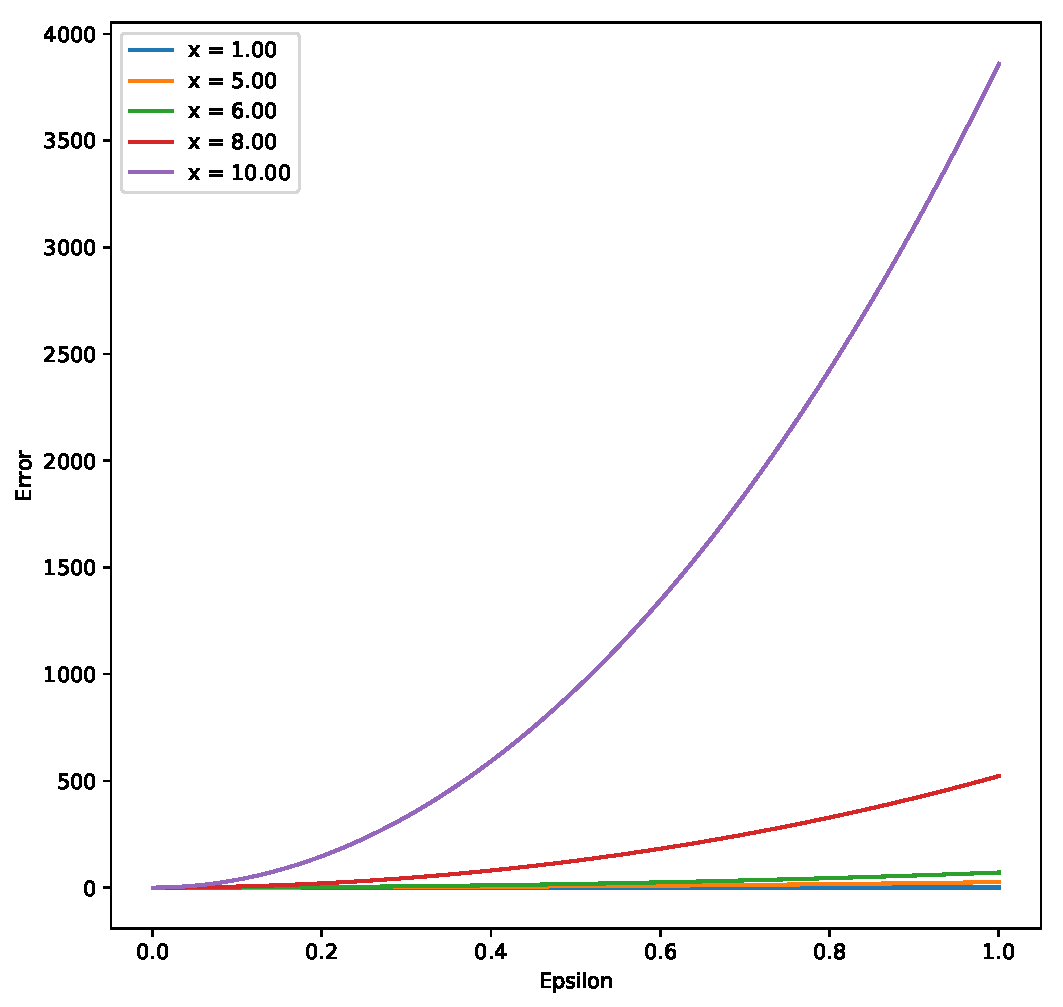
\includegraphics[scale=.9]{plot.pdf}
			\caption{Fig 1. Error values as a function of epsilon for different values of x}
		\end{figure}
\end{enumerate}
\end{document}
